% Options for packages loaded elsewhere
\PassOptionsToPackage{unicode}{hyperref}
\PassOptionsToPackage{hyphens}{url}
\PassOptionsToPackage{dvipsnames,svgnames,x11names}{xcolor}
\documentclass[
  letterpaper,
  oneside,
  11pt,
  openany]{scrbook}
\usepackage{xcolor}
\usepackage[margin=0.9in,headheight=14pt]{geometry}
\usepackage{amsmath,amssymb}
\setcounter{secnumdepth}{-\maxdimen} % remove section numbering
\usepackage{iftex}
\ifPDFTeX
  \usepackage[T1]{fontenc}
  \usepackage[utf8]{inputenc}
  \usepackage{textcomp} % provide euro and other symbols
\else % if luatex or xetex
  \usepackage{unicode-math} % this also loads fontspec
  \defaultfontfeatures{Scale=MatchLowercase}
  \defaultfontfeatures[\rmfamily]{Ligatures=TeX,Scale=1}
\fi
\usepackage{lmodern}
\ifPDFTeX\else
  % xetex/luatex font selection
\fi
% Use upquote if available, for straight quotes in verbatim environments
\IfFileExists{upquote.sty}{\usepackage{upquote}}{}
\IfFileExists{microtype.sty}{% use microtype if available
  \usepackage[]{microtype}
  \UseMicrotypeSet[protrusion]{basicmath} % disable protrusion for tt fonts
}{}
\makeatletter
\@ifundefined{KOMAClassName}{% if non-KOMA class
  \IfFileExists{parskip.sty}{%
    \usepackage{parskip}
  }{% else
    \setlength{\parindent}{0pt}
    \setlength{\parskip}{6pt plus 2pt minus 1pt}}
}{% if KOMA class
  \KOMAoptions{parskip=half}}
\makeatother
\usepackage{longtable,booktabs,array}
\usepackage{calc} % for calculating minipage widths
% Correct order of tables after \paragraph or \subparagraph
\usepackage{etoolbox}
\makeatletter
\patchcmd\longtable{\par}{\if@noskipsec\mbox{}\fi\par}{}{}
\makeatother
% Allow footnotes in longtable head/foot
\IfFileExists{footnotehyper.sty}{\usepackage{footnotehyper}}{\usepackage{footnote}}
\makesavenoteenv{longtable}
\usepackage{graphicx}
\makeatletter
\newsavebox\pandoc@box
\newcommand*\pandocbounded[1]{% scales image to fit in text height/width
  \sbox\pandoc@box{#1}%
  \Gscale@div\@tempa{\textheight}{\dimexpr\ht\pandoc@box+\dp\pandoc@box\relax}%
  \Gscale@div\@tempb{\linewidth}{\wd\pandoc@box}%
  \ifdim\@tempb\p@<\@tempa\p@\let\@tempa\@tempb\fi% select the smaller of both
  \ifdim\@tempa\p@<\p@\scalebox{\@tempa}{\usebox\pandoc@box}%
  \else\usebox{\pandoc@box}%
  \fi%
}
% Set default figure placement to htbp
\def\fps@figure{htbp}
\makeatother
\setlength{\emergencystretch}{3em} % prevent overfull lines
\providecommand{\tightlist}{%
  \setlength{\itemsep}{0pt}\setlength{\parskip}{0pt}}
% Fonts: Charter for text, Helvetica Neue for headings, Menlo for code.
% Charter lacks arrows and a few symbols, so text falls back to Menlo for them.
\directlua{luaotfload.add_fallback("algofallback", {"Menlo:mode=harf;"})}
\setmainfont{Charter}[RawFeature={fallback=algofallback}]
\setsansfont{Helvetica Neue}[RawFeature={fallback=algofallback}]
\setmonofont{Menlo}[Scale=0.86]

\usepackage{xcolor}
\definecolor{accent}{HTML}{1F3A93}
\definecolor{muted}{HTML}{6B7280}
\definecolor{rulegray}{HTML}{B9C0CC}
\definecolor{ink}{HTML}{1D2433}

\setkomafont{disposition}{\normalcolor\sffamily\bfseries\color{accent}}
\setkomafont{section}{\Large}
\setkomafont{chapter}{\huge}
\RedeclareSectionCommand[beforeskip=0pt,afterskip=0.35em]{section}

% Code and pictures: framed verbatim boxes that wrap if ever too long.
\usepackage{fvextra}
\DefineVerbatimEnvironment{PictureVerb}{Verbatim}{frame=single,framesep=2.5mm,rulecolor=\color{rulegray},fontsize=\small,breaklines=true}

% Running heads: tier on the left, entry on the right, page number below.
\usepackage{scrlayer-scrpage}
\manualmark
\clearpairofpagestyles
\ihead{\leftmark}
\ohead{\rightmark}
\cfoot*{\pagemark}
\setkomafont{pageheadfoot}{\normalfont\sffamily\footnotesize\color{muted}}

\newcommand{\entrymeta}[1]{{\sffamily\small\color{muted}#1\par}\vspace{0.6em}}

\setlength{\parindent}{0pt}
\setlength{\parskip}{0.6em plus 0.2em}
\widowpenalty=10000
\clubpenalty=10000
\raggedbottom

% Room for three-digit page numbers in the table of contents.
\makeatletter
\renewcommand*\@pnumwidth{2.2em}
\makeatother
\usepackage{bookmark}
\IfFileExists{xurl.sty}{\usepackage{xurl}}{} % add URL line breaks if available
\urlstyle{same}
\hypersetup{
  pdftitle={50 System Designs},
  colorlinks=true,
  linkcolor={accent},
  filecolor={Maroon},
  citecolor={Blue},
  urlcolor={accent},
  pdfcreator={LaTeX via pandoc}}

\title{50 System Designs}
\usepackage{etoolbox}
\makeatletter
\providecommand{\subtitle}[1]{% add subtitle to \maketitle
  \apptocmd{\@title}{\par {\large #1 \par}}{}{}
}
\makeatother
\subtitle{Ordered by Importance for System Design Interviews}
\author{}
\date{Requirements · Estimates · API · Data Model · Architecture · Deep
Dives}

\begin{document}
\frontmatter
\maketitle

{
\hypersetup{linkcolor=ink}
\setcounter{tocdepth}{1}
\tableofcontents
}
\mainmatter
\chapter{How to Read This Book}\label{how-to-read}

\markboth{How to Read This Book}{}

This book holds fifty system designs in the order to learn them. The
order is importance for a system design interview: how often the design
is asked, how many other designs reuse its ideas, and how badly a gap in
it shows. Tier 1, the first seventeen, are the designs to know cold.
Tier 2, the next seventeen, are very common. Tier 3, the last sixteen,
are good to know and are where an interview goes when it wants depth.

Every chapter follows the same template, which is also the shape of a
good interview. It opens with the system and the two or three questions
that decide its design. Then come the requirements, functional and
non-functional, with the numbers that matter; back-of-the-envelope
estimates, each derivation on its own line; the API; the data model; and
the high-level architecture as a diagram, followed by a walk through its
main paths. Two or three deep dives take on the genuinely hard parts.
The chapter closes with scaling and bottlenecks, failure modes,
trade-offs and alternatives, and the follow-up questions interviewers
actually ask, with crisp answers. The last line lists the algorithms the
design uses.

A reference such as \#139 points to entry 139 of the companion books,
\emph{150 Algorithms in Pseudocode} and \emph{150 Algorithms in Python},
where consistent hashing is explained down to the code. A reference such
as Chapter \hyperref[d5]{5} points to another design in this book and is
a link.

In a 45-minute interview, spend about five minutes on requirements and
estimates, five to eight on the API and data model, ten on the
architecture, fifteen on two deep dives, and the rest on scaling,
failures and trade-offs. The chapters give you more than you can say in
that time on purpose: the interviewer chooses the deep dives, and you
should be ready for any of them.

\section{Reading the Diagrams}\label{reading-the-diagrams}

Every architecture diagram uses the same shapes. Solid arrows are
synchronous calls on the request path; dashed arrows are asynchronous
flows such as events on a queue.

\begin{center}

\pandocbounded{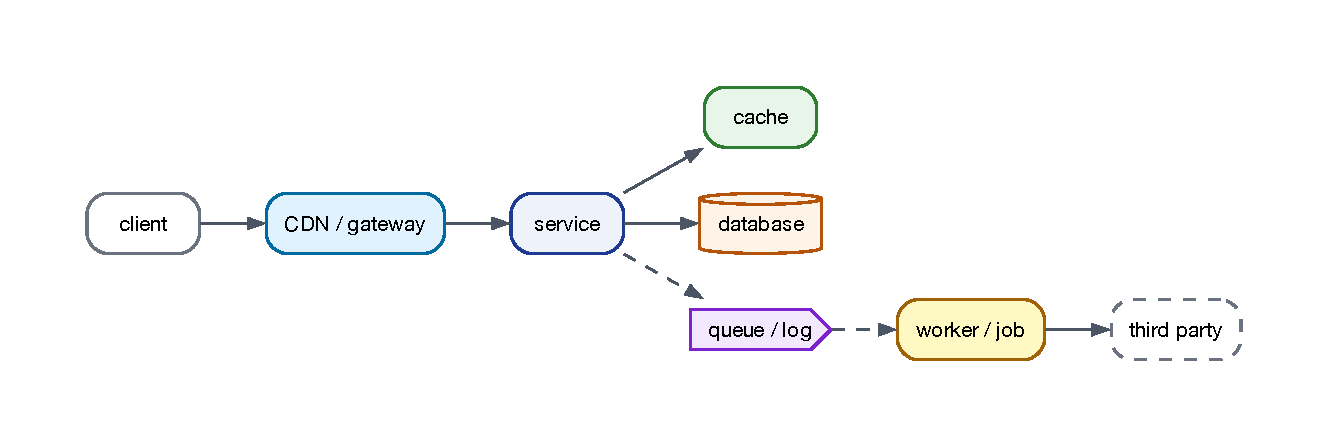
\includegraphics[keepaspectratio]{diagrams/46b1f2c143ec1228.pdf}}

\end{center}

\section{Numbers Worth Knowing}\label{numbers-worth-knowing}

Estimates only need to be right to within a factor of a few, so a
handful of conversions carry most of them. A day has 86,400 seconds,
close enough to 10\^{}5, and peak traffic usually runs two to three
times the daily average.

\begin{PictureVerb}
TRAFFIC                                  STORAGE
1 M requests/day   ≈ 12 per second       2^10 ≈ 10^3   kilo
100 M per day      ≈ 1,200 per second    2^20 ≈ 10^6   mega
1 B per day        ≈ 12,000 per second   2^30 ≈ 10^9   giga
peak               ≈ 2-3 × average       2^40 ≈ 10^12  tera
                                         2^50 ≈ 10^15  peta

LATENCY (the classic table, rounded)
L1 cache reference                       0.5 ns
main memory reference                    100 ns
send 1 KB over a 1 Gbps network          10 µs
read 4 KB at random from SSD             150 µs
read 1 MB sequentially from memory       250 µs
round trip inside a data centre          500 µs
read 1 MB sequentially from SSD          1 ms
disk seek                                10 ms
read 1 MB sequentially from disk         20 ms
packet from California to Europe and back  150 ms
\end{PictureVerb}

Modern hardware has shrunk the memory and SSD rows several times over,
but the ratios still hold, and they are what a design needs: memory is
about a thousand times faster than a network round trip, a round trip
inside a data centre is hundreds of times faster than one across an
ocean, and sequential reads beat random ones everywhere.

\chapter{Tier 1 · Must Know}\label{tier1}

\markboth{Tier 1 · Must Know}{}

These seventeen designs are the ones interviewers reach for first. Each
is a family of its own: the read-heavy service behind a cache, the
limiter in front of every API, the partitioned and replicated store, the
cache cluster, the feed, the chat system and its multi-device cousin,
video upload and streaming, file sync, collaborative editing, the
distributed log, geospatial matching and routing, the CDN, autocomplete
and the crawler. Know them well enough to run each interview end to end
without notes.

\clearpage

\section{1. URL Shortener}\label{d1}

\markright{1. URL Shortener}

{\sffamily\small\color{muted}Base62 IDs, a Read-Heavy Cache, 301 vs 302
· Tier 1}

A URL shortener turns a long link into a short one,
\texttt{https://sho.rt/3fZk9Qa}, and sends everyone who opens the short
link on to the original. The write side is small and simple. The read
side is huge, sensitive to latency and almost perfectly cacheable,
because a short link never changes its target. Three questions decide
the design: how to mint codes that never collide, how to answer a
hundred thousand redirects a second from memory, and which HTTP redirect
to send back.

\subsection{Requirements}\label{requirements}

A user submits a long URL and receives a short code; they may ask for a
custom alias and an expiry date. Anyone who opens the short link is
redirected to the long URL, and the owner can see how many times it was
clicked, day by day. A link is immutable once created: its target never
changes, and the whole read path leans on that property.

The non-functional requirements matter more than the features. A
redirect must complete in well under 100 ms at the 99th percentile,
because it sits in front of somebody else's page. Redirects must stay
available even when the write path is down, since a broken short link
printed in an advert or a QR code cannot be fixed by the person holding
it. Codes must be unique forever, and links must survive for years.
Click counts may lag by a minute and may be approximate. Accounts,
billing, editing a link's target and link-in-bio pages are out of scope.

\subsection{Estimates}\label{estimates}

\begin{PictureVerb}
new links    100 M per day / 86,400 s  ≈ 1,200 writes/s  (peak ×3: 3,500/s)
redirects    100 reads per write       ≈ 120,000 reads/s (peak ×3: 350,000/s)
record       code 7 B + URL ~100 B + owner, dates, flags → round up to 500 B
storage      100 M × 365 × 10 years = 365 B links × 500 B ≈ 180 TB
code space   62^7 ≈ 3.5 × 10^12 codes ≈ 10 × all the links of ten years
hot set      ~50 M links clicked on a given day × 500 B ≈ 25 GB per region
\end{PictureVerb}

Two numbers shape everything that follows. Reads outnumber writes a
hundred to one, so the read path has to be served from memory and the
database only backs up the misses. Ten years of links come to a couple
of hundred terabytes, too much for one machine and comfortable for a
partitioned key-value store. Seven base62 characters give 3.5 trillion
codes, ten times the links the service will ever hold, so codes stay at
seven characters for its whole life. And the hot set, the links that
anyone clicks on a given day, fits in the memory of a small cache
cluster in every region.

\subsection{API}\label{api}

\begin{PictureVerb}
POST /api/v1/links                         Idempotency-Key: <uuid>
     {"long_url": "https://...", "alias": "spring-sale", "expires_at": "..."}
     201 {"code": "3fZk9Qa", "short_url": "https://sho.rt/3fZk9Qa"}
     400 invalid or blocked URL      409 alias already taken

GET  /{code}
     302 Location: <long_url>        404 unknown code       410 expired

GET  /api/v1/links/{code}/stats?from=2026-10-01&to=2026-10-07
     200 {"total": 18234, "by_day": [{"day": "2026-10-01", "clicks": 2511}]}
\end{PictureVerb}

The create call carries an \texttt{Idempotency-Key} header. A client
that times out and retries gets the same code back instead of a second
link, because the server keeps each key with its response for a day. The
redirect endpoint is deliberately bare: no authentication, no body, one
lookup, which is exactly what lets a CDN cache it. Statistics live
behind a separate, authenticated endpoint that reads a different table,
so heavy reporting can never slow a redirect.

\subsection{Data Model}\label{data-model}

\begin{PictureVerb}
links     code PK | long_url | owner_id | created_at | expires_at | status
          partitioned by hash(code), 3 replicas
clicks    (code, day) PK | count          written only by the aggregation job
by_owner  (owner_id, created_at) PK → code      optional, for "my links"
\end{PictureVerb}

Every redirect is a lookup by primary key and nothing ever joins, so a
key-value or wide-column store such as DynamoDB, Cassandra or Bigtable
fits better than a relational database at this scale. Partitioning by a
hash of the code spreads both data and load evenly; partitioning by
owner would pile a large customer's millions of links onto one
partition. A custom alias is simply a code the user chose, stored in the
same table, so one conditional write enforces uniqueness for generated
codes and aliases alike. The \texttt{status} column lets an abuse team
disable a link without deleting its record. Click counts never touch the
links table: redirects emit events and an aggregation job writes daily
totals into \texttt{clicks}. The \texttt{by\_owner} table, kept up to
date off the hot path, serves the page where users see their own links.

\subsection{Architecture}\label{architecture}

\begin{center}

\pandocbounded{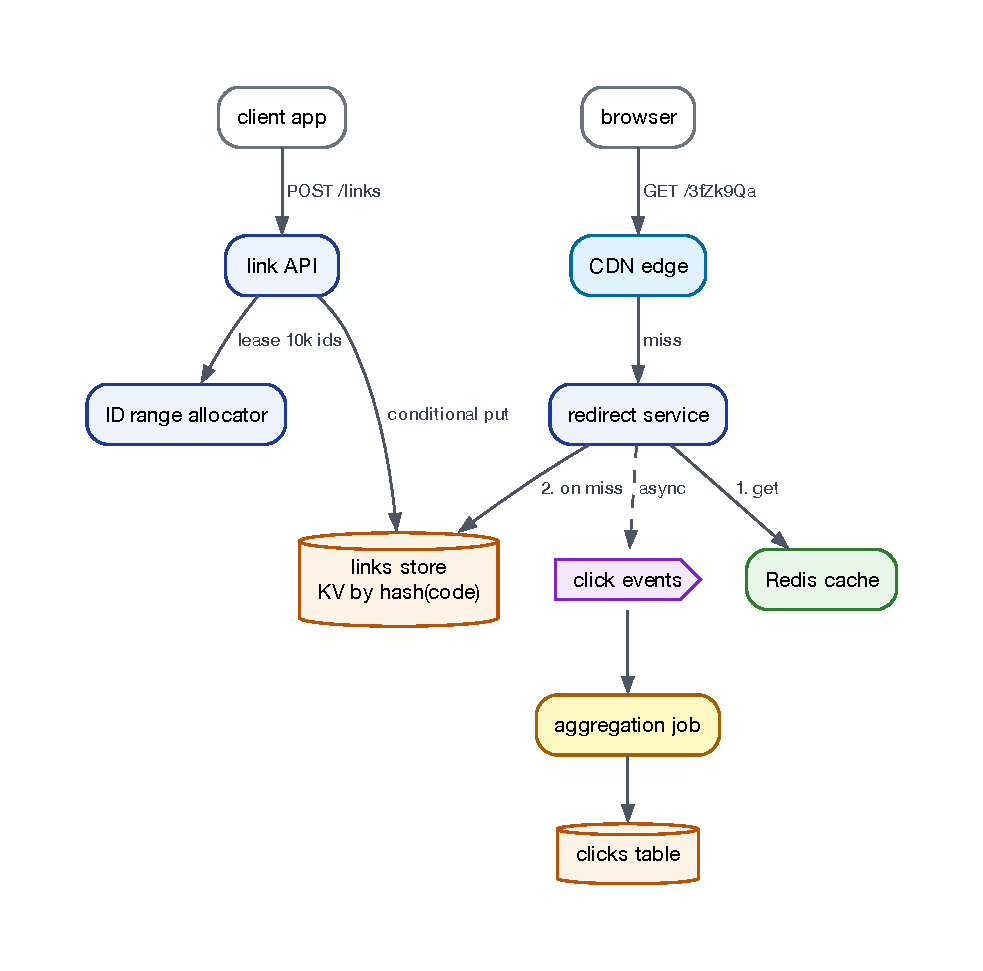
\includegraphics[keepaspectratio]{diagrams/40ed04faf69b23a8.pdf}}

\end{center}

The write path starts at the client app. The link API validates the long
URL (scheme, length, a check against lists of known malicious domains)
and honours the idempotency key. It then takes the next number from the
block of ids it has leased, turns it into seven base62 characters and
writes the record with a conditional put that fails if the code already
exists. Only after that write succeeds does it answer 201.

The read path starts at the browser. The CDN edge answers at once if it
holds a cached response for \texttt{/3fZk9Qa}, usually from a city near
the user. On a miss the request reaches a stateless redirect service,
which looks the code up in a Redis cluster and, on a miss there, reads
the links store and fills the cache. It returns the redirect and,
without waiting, drops a click event on a queue that an aggregation job
rolls up into per-day counts. Each layer absorbs most of the traffic
that reaches it, so the store sees only a small fraction of all
redirects.

\subsection{Deep Dives}\label{deep-dives}

\subsubsection{Minting codes that never
collide}\label{minting-codes-that-never-collide}

The tempting idea is to hash the long URL with MD5 or SHA-256 and keep
the first seven base62 characters. The same URL then always gets the
same code, which deduplicates for free. But seven characters hold only
about 42 bits, and the birthday bound is merciless: with \texttt{n}
links in a space of \texttt{N} codes, the expected number of colliding
pairs is about \texttt{n²\ /\ 2N}, and for a single year of links (3.65
× 10\^{}10) that is already around 190 million. Every write would have
to read before it writes and retry with a salt on a collision, and the
retries pile up as the table fills.

A counter cannot collide. Number the links 1, 2, 3 and write each number
in base62. A single counter, though, is a bottleneck and a single point
of failure, so the counter is handed out in ranges. Each API server asks
a small coordination store, a row updated with compare-and-set or a key
in ZooKeeper or etcd, for the next block of 10,000 numbers and then
counts through its block in memory. At 3,500 writes a second the
coordination store sees one request every few seconds. A server that
crashes loses the rest of its block, which leaves a gap in the sequence
and costs nothing else.

Sequential codes have one weakness: they are guessable, so anyone can
enumerate every link by counting. Scramble the number before encoding it
with a bijection on the code space, for example by multiplying it by a
large secret constant that shares no factor with 62\^{}7 and taking the
result modulo 62\^{}7. The mapping stays one-to-one, so uniqueness
survives, but neighbouring numbers land far apart. A 64-bit
Snowflake-style id (\#145) needs no coordination at all, yet it takes
eleven base62 characters, which is why shorteners prefer a leased
counter. Custom aliases go through the same conditional write, and if a
generated code ever lands on an existing alias, the put fails and the
server simply takes the next number in its block.

\subsubsection{The redirect path: caching, and 301 versus
302}\label{the-redirect-path-caching-and-301-versus-302}

Because a link never changes, a cached answer never goes stale; only
expiry and an abuse takedown invalidate it. Caching is therefore nearly
free of the usual consistency trouble. The CDN edge caches the redirect
response itself for a few minutes, Redis caches code-to-URL mappings
with LRU eviction (\#44), and the store is the source of truth. A viral
link is the classic hot key, millions of requests for one code. The CDN
absorbs most of them, and the redirect service coalesces concurrent
misses for the same code into a single store read, so a link that goes
viral in its first minute does not stampede the database. Unknown codes
are cached too, briefly, as negative entries, so a bot scanning random
codes hits Redis instead of the store.

The status code is a product decision dressed up as a protocol detail. A
301 (Moved Permanently) lets browsers and proxies cache the redirect
indefinitely. Repeat visits then never reach the service, the cheapest
read path there is, but those clicks vanish from the analytics, and
expiry or a takedown cannot reach a browser that has already cached the
answer. A 302 (Found), or its stricter cousin 307, asks the client to
come back every time, which keeps analytics complete and makes expiry
and takedowns work immediately, at the price of serving every click.
This design returns 302 and lets the CDN cache it for a few minutes with
an explicit \texttt{Cache-Control} header, and the CDN's access logs
report the clicks it served. A service that only shortens permanent
links and sells no analytics should choose 301.

\subsubsection{Counting clicks without slowing
redirects}\label{counting-clicks-without-slowing-redirects}

A redirect never waits on analytics. The redirect service hands a small
event (code, timestamp, country, referrer) to a local buffer that ships
to a Kafka topic; if the pipeline is slow, events are dropped rather
than redirects delayed, which approximate counts can afford. A stream
job aggregates events per code per minute and writes daily totals.
Counting in the job instead of the database also solves the write side
of the hot-key problem: a viral link generates millions of increments
that no single counter row could absorb, and the job folds them into one
write per minute. Exactly-once counting is unnecessary for a dashboard;
if clicks are ever billed, every event carries an id and the job
deduplicates within its window.

\subsection{Scaling and Bottlenecks}\label{scaling-and-bottlenecks}

Every tier of the read path scales horizontally. Redirect servers are
stateless and sit behind a load balancer. The Redis cluster shards codes
with consistent hashing (\#139), so adding a node moves only a slice of
the keys, and replicas absorb reads of the hottest ones. The store
partitions by a hash of the code and keeps three replicas. The write
path stopped being a bottleneck the moment ids were leased in blocks,
because the allocator sees one request per block rather than one per
link.

Going multi-region is mostly about reads. Each region runs its own CDN
presence, redirect fleet, cache and a replica of the links store,
replicated asynchronously from the region that created the link. Because
links never change, eventual consistency has exactly one visible effect:
a link created in Europe may not exist in Asia for a second or two. The
creating region writes through its own cache, and a remote region that
misses can ask the home region before answering 404, which closes the
gap. What remains is a cold cache after a failover or a large
deployment, which the next section deals with.

\subsection{Failure Modes}\label{failure-modes}

If the cache cluster fails, every redirect falls through to the store,
which is sized for misses rather than for the full load. Request
coalescing, a rate limiter in front of the store (\#138) and a warm
standby cache keep that from becoming an outage, and letting the CDN
serve stale entries for longer buys time. If the ID allocator goes down,
API servers keep minting codes from the blocks they already hold; blocks
sized to cover an hour of writes turn an allocator outage into a
non-event. A crashed API server simply loses its block, and a failed
store replica is covered by the other two and by quorum reads.

Retried creates are absorbed by the idempotency key, and a failure
between the conditional put and the response leaves a valid link that
the retry finds through that key. A region failure is handled by DNS or
anycast steering users to the next region, whose replica already holds
almost every link. The quieter failure is abuse. Shorteners are a
favourite tool for hiding phishing pages, so links are checked against
reputation lists when they are created and rescanned later, and a
takedown sets \texttt{status}, deletes the cache entry and purges the
CDN.

\subsection{Trade-offs and
Alternatives}\label{trade-offs-and-alternatives}

The central trade is how codes are made. A counter guarantees uniqueness
and the shortest possible codes, and pays with a coordination store and
a scrambling step. Hashing the URL needs no coordination and
deduplicates identical links, and pays with a read before every write
and retries that grow as the table fills. Many products want
deduplication only per user, which the counter design gets cheaply from
a per-owner index on a hash of the long URL. The storage choice is less
dramatic than it looks: below a few billion links, one relational
database with an auto-increment key and read replicas is simpler and
entirely adequate, and its primary key becomes the counter.

The redirect code trades offload against control, as the deep dive
showed, and counting clicks asynchronously trades a minute of lag for
redirects that never wait on a write. Code length is the last dial.
Seven characters last a decade at this rate, and every extra character
buys sixty-two times the space for a slightly longer link.

\subsection{What Interviewers Probe}\label{what-interviewers-probe}

Expect the conversation to circle five questions. How do you guarantee
unique codes across many servers? Lease ranges of a counter from a
coordination store and accept gaps on a crash. How long is a code, and
why? Show the 62\^{}7 arithmetic against ten years of links. What
happens when a link goes viral? The CDN, the cache, request coalescing,
and negative caching for scanners. Do you return 301 or 302? Explain the
trade between offload and analytics and pick one deliberately. How do
you count clicks at 100,000 a second without slowing redirects?
Asynchronous events aggregated by a stream job.

Strong candidates raise three more points unprompted: enumeration, which
a scrambled counter prevents; abuse, which needs reputation checks and
fast takedowns; and multiple regions, where immutable links make
asynchronous replication safe. Interviewers rarely care which database
brand you pick. They care that the common-case read never touches the
database at all.

\emph{Algorithms:} \#100 URL Shortener · \#145 Unique ID Generator ·
\#139 Consistent Hashing · \#44 LRU Cache · \#138 Rate Limiter

\clearpage

\chapter{Where the Algorithms Appear}\label{algorithm-index}

\markboth{Where the Algorithms Appear}{}

Each algorithm from \emph{150 Algorithms} that a design in this book
relies on, with the chapters that use it. Chapter numbers are links.

\begin{longtable}[]{@{}
  >{\raggedright\arraybackslash}p{(\linewidth - 2\tabcolsep) * \real{0.4125}}
  >{\raggedright\arraybackslash}p{(\linewidth - 2\tabcolsep) * \real{0.5875}}@{}}
\toprule\noalign{}
\begin{minipage}[b]{\linewidth}\raggedright
Algorithm
\end{minipage} & \begin{minipage}[b]{\linewidth}\raggedright
Used in
\end{minipage} \\
\midrule\noalign{}
\endhead
\bottomrule\noalign{}
\endlastfoot
\#44 LRU Cache & Chapter \hyperref[d1]{1} URL Shortener \\
\#100 URL Shortener & Chapter \hyperref[d1]{1} URL Shortener \\
\#138 Rate Limiter & Chapter \hyperref[d1]{1} URL Shortener \\
\#139 Consistent Hashing & Chapter \hyperref[d1]{1} URL Shortener \\
\#145 Unique ID Generator & Chapter \hyperref[d1]{1} URL Shortener \\
\end{longtable}

\backmatter
\end{document}
